% !TEX root = ../dissertation.tex

\chapter{Sancho Overview}
\label{chapter:sancho_overview}

A more up to date and detailed overview of the Sancho project is given in this chapter

\section{The overall architecture}

Sancho is based on the ggp-base framework.
It spawns many different threads but there are only 3 important types:
\begin{itemize}
	\item 1 HTTP server thread: Responsible for network communication with the game manager.
	\item 1 MCTS structure control thread: Handles all MCTS steps except simulation. It's the only thread that can modify the MCTS graph.
	\item N Playout threads: These threads handle simulations (random playouts).    
\end{itemize}
	
\todo[inline]{make diagram}
	
\begin{figure}[h]
	\centering
	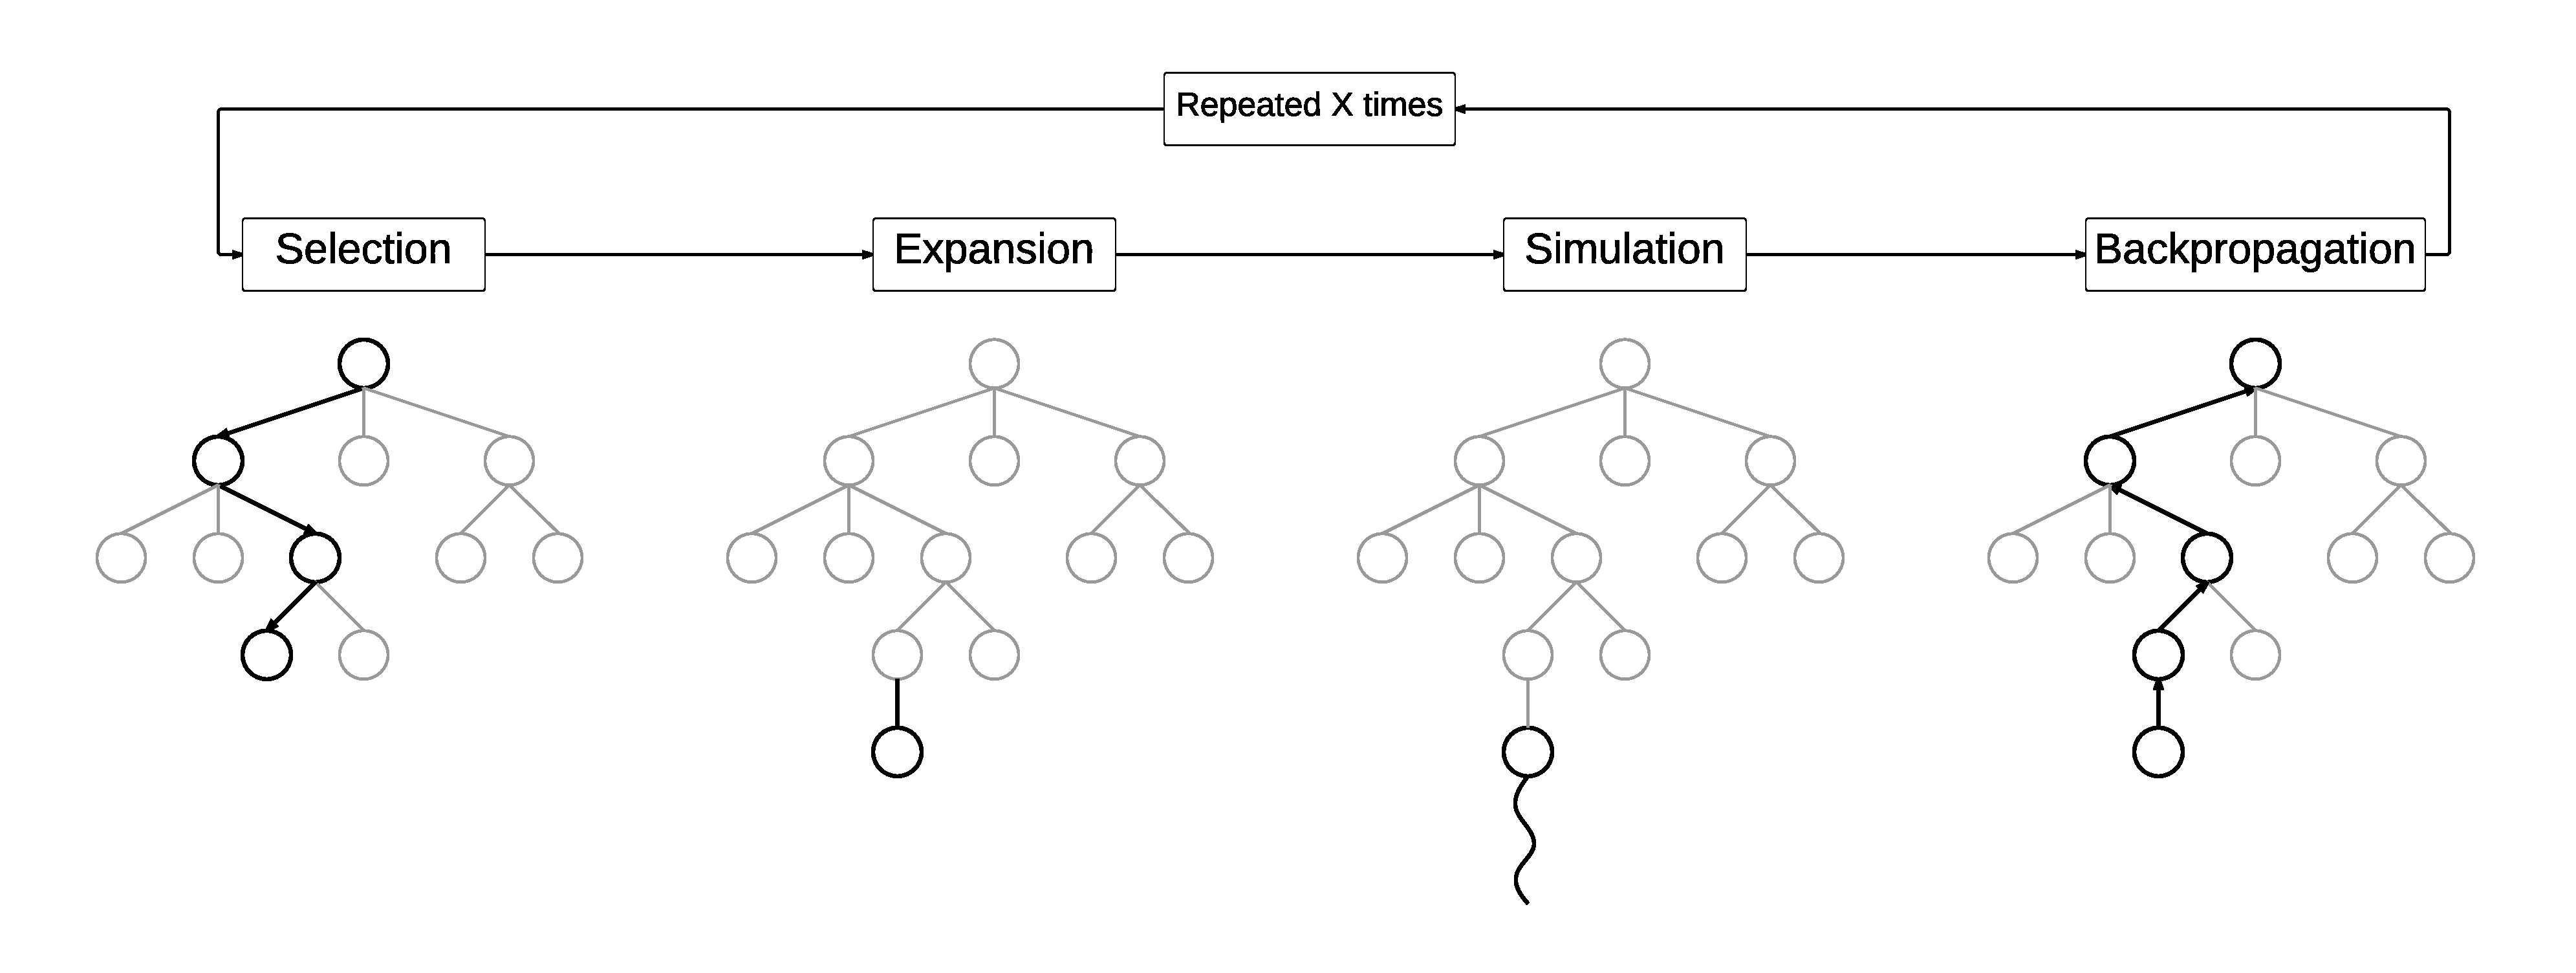
\includegraphics[width=\textwidth]{images/MCTS.pdf}
%	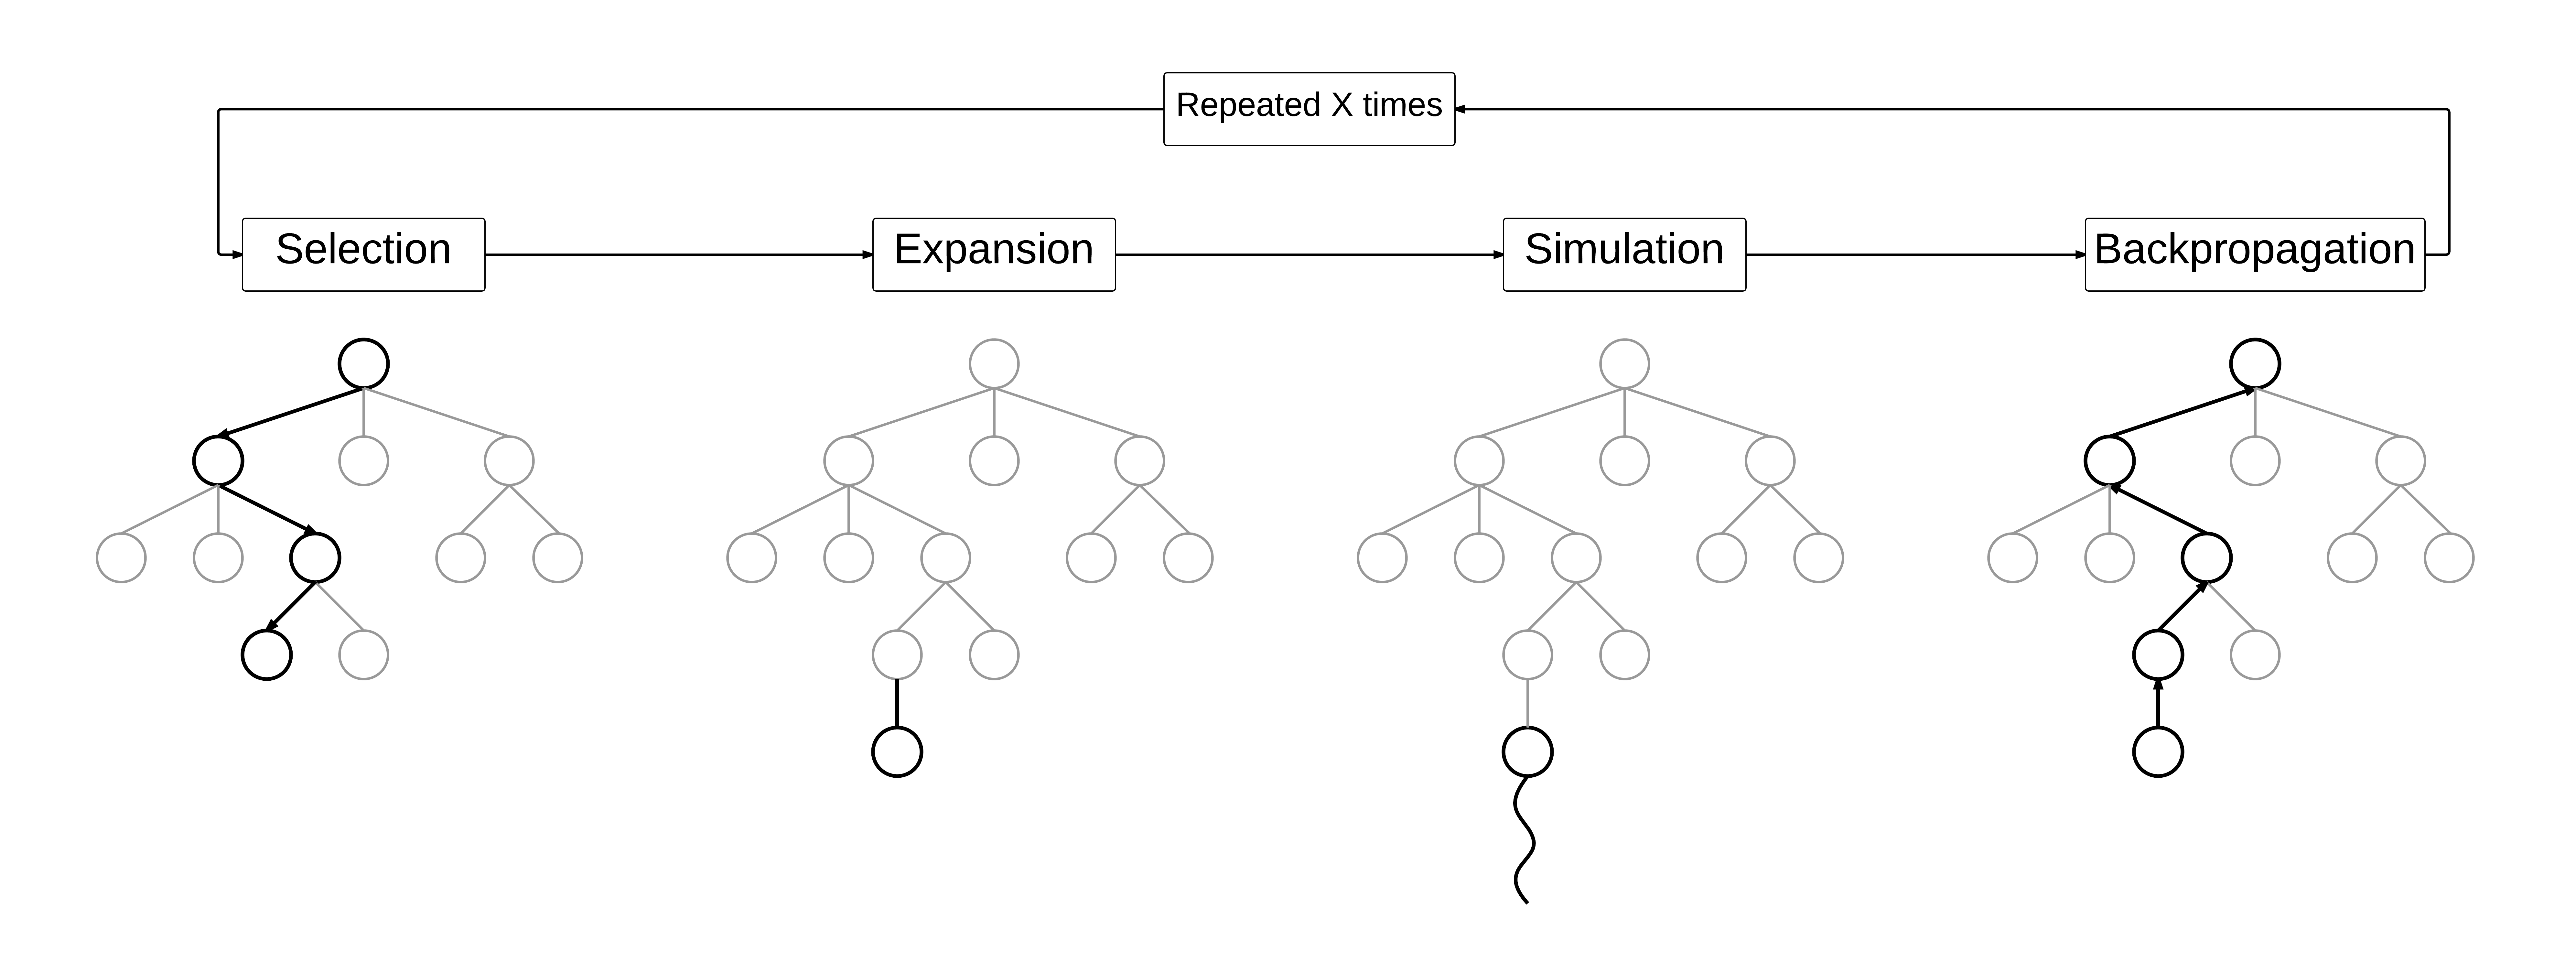
\includegraphics[width=\textwidth]{images/MCTS.png}
	\caption{MCTS steps}
	\label{fig:mcts steps}
\end{figure}


\section{Meta-Gaming}

\subsection{Heuristics}

\section{Propositional Networks Implementation}

\section{1-player games (puzzles) solving}



